\section{Generalized Gamma Algebra for Fat Tails}

\begin{frame}{High-level Idea}
    \begin{figure}
        \centering
        \resizebox{\columnwidth}{!}{%
        
            % \begin{tblr}{colspec={Q[.4\textwidth]Q[.2\textwidth]Q[.3\textwidth]}}
            % \centering \bf Analyze Target & \centering \bf Calibrate Tails & \centering \bf Refine Bulk
            % \end{tblr}~\\
            % \vspace{-1.2cm}
            
            {
            \SetTblrInner{rowsep=-8pt}
            \begin{tblr}{colspec={c Q[.15cm] c Q[1.1cm] c Q[.15cm] c},columns={m,m,m,m,m,m,m}}
            %\centering Code & & \centering Computation Graph & & \centering Tail Class & & \centering Normalizing Flow
            %\\
            \raisebox{-.5\height}{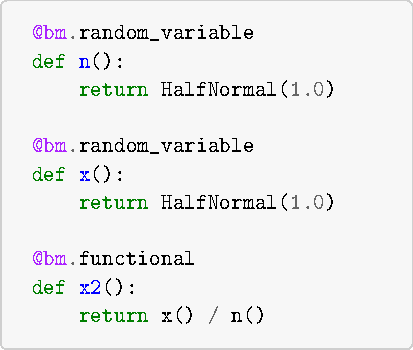
\includegraphics[width=0.25\textwidth]{Figures/gga/schematic_code.pdf} \hspace{-.3cm}}
            &\scalebox{1}{$\boldsymbol{\longrightarrow}$} & \raisebox{-.4\height}{\hspace{-.3cm} 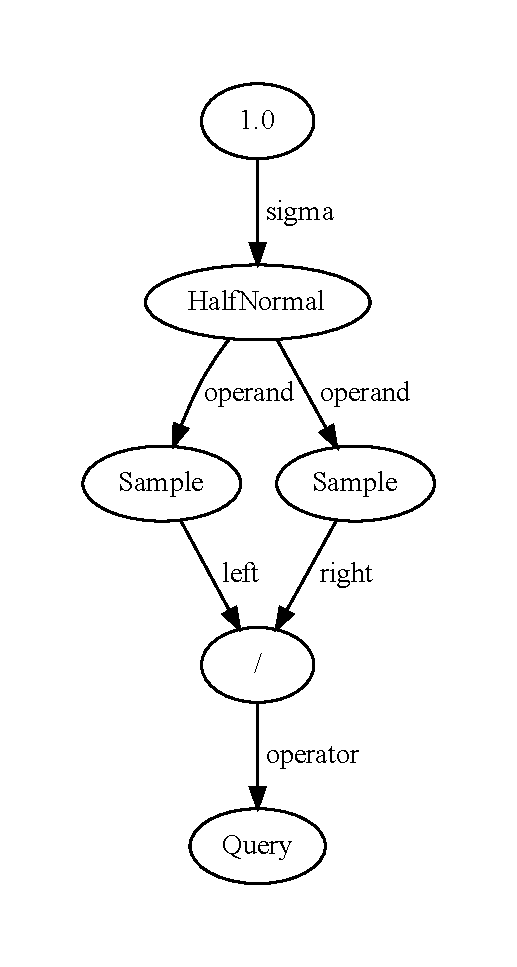
\includegraphics[width=0.2\textwidth]{Figures/gga/schematic.gv.pdf}\hspace{-.2cm}} & \hspace{-.5cm}\scalebox{1.7}{$\xrightarrow{\,\,\textit{\textbf{GGA}}\,\,}$}\hspace{-.7cm}  &  \stackanchor{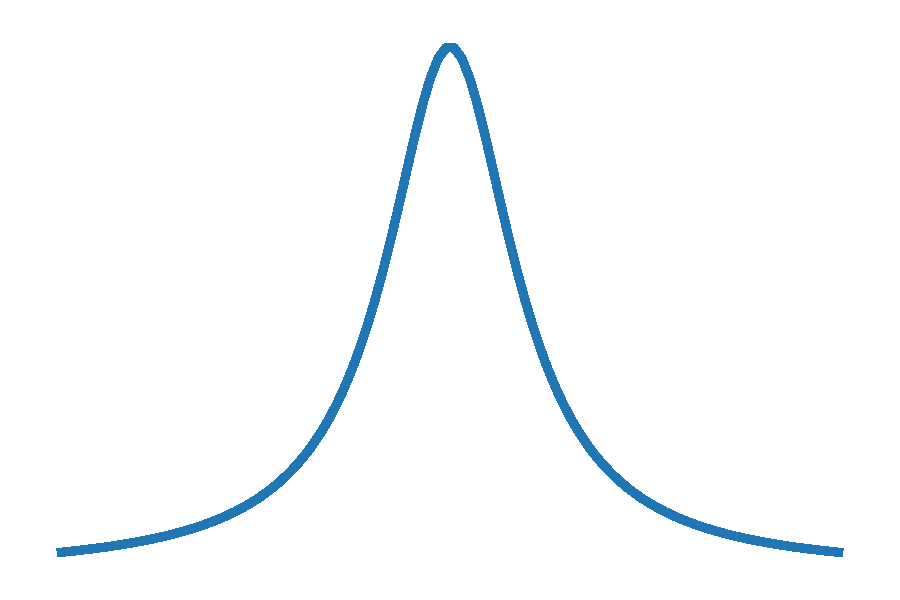
\includegraphics[width=0.15\textwidth]{Figures/gga/schematic_cauchy.pdf}}{\scalebox{3}{$\mathcal{R}_2$}}\hspace{-.3cm} & \scalebox{1}{$\boldsymbol{\longrightarrow}$ } & \raisebox{-.5\height}{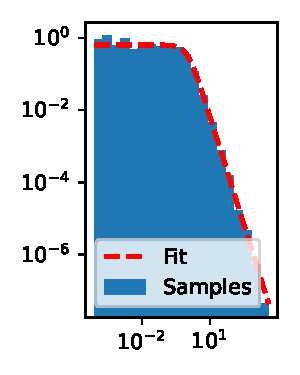
\includegraphics[width=0.2\textwidth]{Figures/gga/schematic_final.pdf}} \\
            (1) & & (2) & & (3) & & (4)
            \end{tblr}
            }
    
        }
    \end{figure}
\end{frame}

\begin{frame}{Generalized gamma tail parameterization}
    \begin{definition}
        Let $\nu \in \mathbb{R}$, $\sigma > 0$, and $\rho \in \mathbb{R} \backslash \{0\}$ be such that $(\nu+1)/ \rho > 0$.
        A non-negative random variable $X$ is \emph{generalized Gamma distributed} with parameters $\nu,\sigma,\rho$ if it has Lebesgue density
        \begin{equation}
        \label{eq:GenGammaDensity}
        p_{\nu,\sigma,\rho}(x) = c_{\nu,\sigma,\rho} x^\nu e^{-\sigma x^\rho},\qquad x > 0,
        \end{equation}
        where $c_{\nu,\sigma,\rho} = \rho \sigma^{(\nu+1)/\rho} / \Gamma((\nu+1)/\rho)$ is the normalizing constant. %The generalized Gamma density incorporates many other well-known densities, including that of the Gamma distribution ($\rho = 1$), and the Frechet/Weibull distribution ($\nu = \rho - 1$). 
    \end{definition}
\end{frame}

\begin{subframe}{Static analysis in PPL}
    \begin{algorithm}[H]
    	\caption{Pseudocode for a GGA tails static analysis pass}\label{alg:bfs_typecheck}
    	\KwData{Abstract syntax tree for a PPL program}
    	\KwResult{GGA parameter estimates for all random variables}
    	frontier $\gets$ [rv : Parents(rv) = $\emptyset$]\;
    	GGAs $\gets \{\}$\;
    	\While{\text{frontier} $\neq \emptyset$}{
    		next $\gets$ frontier.popLeft()\;
    		GGAs[next] $\gets$ computeGGA(next.op, next.parent)\;
    		frontier $\gets$ frontier + next.children()\;
    	}
    	\Return{GGAs}
    \end{algorithm}
\end{subframe}

\begin{frame}{Prior work}

    \parencite{resnick2007heavy}: closure under addition
    \begin{align*}
        &  (\nu_{1},\sigma_{1},\rho_{1})\oplus(\nu_{2},\sigma_{2},\rho_{2}) \\
        & \equiv \begin{cases}
            \max\{(\nu_{1},\sigma_{1},\rho_{1}),(\nu_{2},\sigma_{2},\rho_{2})\} & \text{ if }\rho_{1}\neq\rho_{2}\text{ or }\rho_{1},\rho_{2}<1\\
            \left(\nu_{1}+\nu_{2}+1,\min\{\sigma_{1},\sigma_{2}\},1\right) & \text{ if }\rho_{1}=\rho_{2}=1\\
            (\nu_{1}+\nu_{2}+\frac{2-\rho}{2},(\sigma_{1}^{-\frac{1}{\rho-1}}+\sigma_{2}^{-\frac{1}{\rho-1}})^{1-\rho},\rho) & \text{ if }\rho=\rho_{1}=\rho_{2}>1.
        \end{cases}
    \end{align*}
\end{frame}

\begin{frame}{New results I\footnote{\fullcite{gga}}}
    Closure under multiplication
    \begin{align*}
        & (\nu_{1},\sigma_{1},\rho_{1})\otimes(\nu_{2},\sigma_{2},\rho_{2}) \\
        &\qquad \equiv\begin{cases}
        \left(\frac{1}{\mu}\left(\frac{\nu_{1}}{|\rho_{1}|}+\frac{\nu_{2}}{|\rho_{2}|}+\frac{1}{2}\right),\sigma,-\frac{1}{\mu}\right) & \text{ if }\rho_{1},\rho_{2}<0\\
        \left(\frac{1}{\mu}\left(\frac{\nu_{1}}{\rho_{1}}+\frac{\nu_{2}}{\rho_{2}}-\frac{1}{2}\right),\sigma,\frac{1}{\mu}\right) & \text{ if }\rho_{1},\rho_{2}>0\\
        \mathcal{R}_{|\nu_1|} & \mbox{ if }\rho_{1}\leq0,\rho_{2}>0 \\
        \mathcal{R}_{\min\{|\nu_1|,|\nu_2|\}} & \mbox{ if }\rho_{1}=0,\rho_{2}=0
        \end{cases} \\
        &\text{where }\mu=\frac{1}{|\rho_{1}|}+\frac{1}{|\rho_{2}|}=\frac{|\rho_{1}|+|\rho_{2}|}{|\rho_{1}\rho_{2}|}, \sigma=\mu(\sigma_{1}|\rho_{1}|)^{\frac{1}{\mu|\rho_{1}|}}(\sigma_{2}|\rho_{2}|)^{\frac{1}{\mu|\rho_{2}|}}.
    \end{align*}
\end{frame}

\begin{frame}{New results II}
    Closure under Lipschitz functions
    \begin{align*}
        & f(X_1,\dots,X_n) \equiv L \max\{X_1,\dots,X_n\}
    \end{align*}
    \pause
    $\therefore$\quad Bulk correction with Lipschitz flow
    \begin{figure}
        \centering
        \resizebox{\textwidth}{!}{
    		%% Creator: Matplotlib, PGF backend
%%
%% To include the figure in your LaTeX document, write
%%   \input{<filename>.pgf}
%%
%% Make sure the required packages are loaded in your preamble
%%   \usepackage{pgf}
%%
%% Also ensure that all the required font packages are loaded; for instance,
%% the lmodern package is sometimes necessary when using math font.
%%   \usepackage{lmodern}
%%
%% Figures using additional raster images can only be included by \input if
%% they are in the same directory as the main LaTeX file. For loading figures
%% from other directories you can use the `import` package
%%   \usepackage{import}
%%
%% and then include the figures with
%%   \import{<path to file>}{<filename>.pgf}
%%
%% Matplotlib used the following preamble
%%
\begingroup%
\makeatletter%
\begin{pgfpicture}%
\pgfpathrectangle{\pgfpointorigin}{\pgfqpoint{5.010654in}{2.322566in}}%
\pgfusepath{use as bounding box, clip}%
\begin{pgfscope}%
\pgfsetbuttcap%
\pgfsetmiterjoin%
\definecolor{currentfill}{rgb}{1.000000,1.000000,1.000000}%
\pgfsetfillcolor{currentfill}%
\pgfsetlinewidth{0.000000pt}%
\definecolor{currentstroke}{rgb}{1.000000,1.000000,1.000000}%
\pgfsetstrokecolor{currentstroke}%
\pgfsetdash{}{0pt}%
\pgfpathmoveto{\pgfqpoint{0.000000in}{0.000000in}}%
\pgfpathlineto{\pgfqpoint{5.010654in}{0.000000in}}%
\pgfpathlineto{\pgfqpoint{5.010654in}{2.322566in}}%
\pgfpathlineto{\pgfqpoint{0.000000in}{2.322566in}}%
\pgfpathlineto{\pgfqpoint{0.000000in}{0.000000in}}%
\pgfpathclose%
\pgfusepath{fill}%
\end{pgfscope}%
\begin{pgfscope}%
\pgfsetbuttcap%
\pgfsetmiterjoin%
\definecolor{currentfill}{rgb}{0.917647,0.917647,0.949020}%
\pgfsetfillcolor{currentfill}%
\pgfsetlinewidth{0.000000pt}%
\definecolor{currentstroke}{rgb}{0.000000,0.000000,0.000000}%
\pgfsetstrokecolor{currentstroke}%
\pgfsetstrokeopacity{0.000000}%
\pgfsetdash{}{0pt}%
\pgfpathmoveto{\pgfqpoint{0.588402in}{0.367514in}}%
\pgfpathlineto{\pgfqpoint{2.320512in}{0.367514in}}%
\pgfpathlineto{\pgfqpoint{2.320512in}{1.995606in}}%
\pgfpathlineto{\pgfqpoint{0.588402in}{1.995606in}}%
\pgfpathlineto{\pgfqpoint{0.588402in}{0.367514in}}%
\pgfpathclose%
\pgfusepath{fill}%
\end{pgfscope}%
\begin{pgfscope}%
\pgfpathrectangle{\pgfqpoint{0.588402in}{0.367514in}}{\pgfqpoint{1.732110in}{1.628093in}}%
\pgfusepath{clip}%
\pgfsetroundcap%
\pgfsetroundjoin%
\pgfsetlinewidth{0.803000pt}%
\definecolor{currentstroke}{rgb}{1.000000,1.000000,1.000000}%
\pgfsetstrokecolor{currentstroke}%
\pgfsetdash{}{0pt}%
\pgfpathmoveto{\pgfqpoint{0.745867in}{0.367514in}}%
\pgfpathlineto{\pgfqpoint{0.745867in}{1.995606in}}%
\pgfusepath{stroke}%
\end{pgfscope}%
\begin{pgfscope}%
\definecolor{textcolor}{rgb}{0.150000,0.150000,0.150000}%
\pgfsetstrokecolor{textcolor}%
\pgfsetfillcolor{textcolor}%
\pgftext[x=0.745867in,y=0.252236in,,top]{\color{textcolor}\sffamily\fontsize{8.800000}{10.560000}\selectfont \(\displaystyle {0}\)}%
\end{pgfscope}%
\begin{pgfscope}%
\pgfpathrectangle{\pgfqpoint{0.588402in}{0.367514in}}{\pgfqpoint{1.732110in}{1.628093in}}%
\pgfusepath{clip}%
\pgfsetroundcap%
\pgfsetroundjoin%
\pgfsetlinewidth{0.803000pt}%
\definecolor{currentstroke}{rgb}{1.000000,1.000000,1.000000}%
\pgfsetstrokecolor{currentstroke}%
\pgfsetdash{}{0pt}%
\pgfpathmoveto{\pgfqpoint{1.533190in}{0.367514in}}%
\pgfpathlineto{\pgfqpoint{1.533190in}{1.995606in}}%
\pgfusepath{stroke}%
\end{pgfscope}%
\begin{pgfscope}%
\definecolor{textcolor}{rgb}{0.150000,0.150000,0.150000}%
\pgfsetstrokecolor{textcolor}%
\pgfsetfillcolor{textcolor}%
\pgftext[x=1.533190in,y=0.252236in,,top]{\color{textcolor}\sffamily\fontsize{8.800000}{10.560000}\selectfont \(\displaystyle {5}\)}%
\end{pgfscope}%
\begin{pgfscope}%
\pgfpathrectangle{\pgfqpoint{0.588402in}{0.367514in}}{\pgfqpoint{1.732110in}{1.628093in}}%
\pgfusepath{clip}%
\pgfsetroundcap%
\pgfsetroundjoin%
\pgfsetlinewidth{0.803000pt}%
\definecolor{currentstroke}{rgb}{1.000000,1.000000,1.000000}%
\pgfsetstrokecolor{currentstroke}%
\pgfsetdash{}{0pt}%
\pgfpathmoveto{\pgfqpoint{2.320512in}{0.367514in}}%
\pgfpathlineto{\pgfqpoint{2.320512in}{1.995606in}}%
\pgfusepath{stroke}%
\end{pgfscope}%
\begin{pgfscope}%
\definecolor{textcolor}{rgb}{0.150000,0.150000,0.150000}%
\pgfsetstrokecolor{textcolor}%
\pgfsetfillcolor{textcolor}%
\pgftext[x=2.320512in,y=0.252236in,,top]{\color{textcolor}\sffamily\fontsize{8.800000}{10.560000}\selectfont \(\displaystyle {10}\)}%
\end{pgfscope}%
\begin{pgfscope}%
\pgfpathrectangle{\pgfqpoint{0.588402in}{0.367514in}}{\pgfqpoint{1.732110in}{1.628093in}}%
\pgfusepath{clip}%
\pgfsetroundcap%
\pgfsetroundjoin%
\pgfsetlinewidth{0.803000pt}%
\definecolor{currentstroke}{rgb}{1.000000,1.000000,1.000000}%
\pgfsetstrokecolor{currentstroke}%
\pgfsetdash{}{0pt}%
\pgfpathmoveto{\pgfqpoint{0.588402in}{0.773926in}}%
\pgfpathlineto{\pgfqpoint{2.320512in}{0.773926in}}%
\pgfusepath{stroke}%
\end{pgfscope}%
\begin{pgfscope}%
\definecolor{textcolor}{rgb}{0.150000,0.150000,0.150000}%
\pgfsetstrokecolor{textcolor}%
\pgfsetfillcolor{textcolor}%
\pgftext[x=0.308967in, y=0.730523in, left, base]{\color{textcolor}\sffamily\fontsize{8.800000}{10.560000}\selectfont \(\displaystyle {0.5}\)}%
\end{pgfscope}%
\begin{pgfscope}%
\pgfpathrectangle{\pgfqpoint{0.588402in}{0.367514in}}{\pgfqpoint{1.732110in}{1.628093in}}%
\pgfusepath{clip}%
\pgfsetroundcap%
\pgfsetroundjoin%
\pgfsetlinewidth{0.803000pt}%
\definecolor{currentstroke}{rgb}{1.000000,1.000000,1.000000}%
\pgfsetstrokecolor{currentstroke}%
\pgfsetdash{}{0pt}%
\pgfpathmoveto{\pgfqpoint{0.588402in}{1.181153in}}%
\pgfpathlineto{\pgfqpoint{2.320512in}{1.181153in}}%
\pgfusepath{stroke}%
\end{pgfscope}%
\begin{pgfscope}%
\definecolor{textcolor}{rgb}{0.150000,0.150000,0.150000}%
\pgfsetstrokecolor{textcolor}%
\pgfsetfillcolor{textcolor}%
\pgftext[x=0.308967in, y=1.137750in, left, base]{\color{textcolor}\sffamily\fontsize{8.800000}{10.560000}\selectfont \(\displaystyle {1.0}\)}%
\end{pgfscope}%
\begin{pgfscope}%
\pgfpathrectangle{\pgfqpoint{0.588402in}{0.367514in}}{\pgfqpoint{1.732110in}{1.628093in}}%
\pgfusepath{clip}%
\pgfsetroundcap%
\pgfsetroundjoin%
\pgfsetlinewidth{0.803000pt}%
\definecolor{currentstroke}{rgb}{1.000000,1.000000,1.000000}%
\pgfsetstrokecolor{currentstroke}%
\pgfsetdash{}{0pt}%
\pgfpathmoveto{\pgfqpoint{0.588402in}{1.588380in}}%
\pgfpathlineto{\pgfqpoint{2.320512in}{1.588380in}}%
\pgfusepath{stroke}%
\end{pgfscope}%
\begin{pgfscope}%
\definecolor{textcolor}{rgb}{0.150000,0.150000,0.150000}%
\pgfsetstrokecolor{textcolor}%
\pgfsetfillcolor{textcolor}%
\pgftext[x=0.308967in, y=1.544977in, left, base]{\color{textcolor}\sffamily\fontsize{8.800000}{10.560000}\selectfont \(\displaystyle {1.5}\)}%
\end{pgfscope}%
\begin{pgfscope}%
\pgfpathrectangle{\pgfqpoint{0.588402in}{0.367514in}}{\pgfqpoint{1.732110in}{1.628093in}}%
\pgfusepath{clip}%
\pgfsetroundcap%
\pgfsetroundjoin%
\pgfsetlinewidth{0.803000pt}%
\definecolor{currentstroke}{rgb}{1.000000,1.000000,1.000000}%
\pgfsetstrokecolor{currentstroke}%
\pgfsetdash{}{0pt}%
\pgfpathmoveto{\pgfqpoint{0.588402in}{1.995606in}}%
\pgfpathlineto{\pgfqpoint{2.320512in}{1.995606in}}%
\pgfusepath{stroke}%
\end{pgfscope}%
\begin{pgfscope}%
\definecolor{textcolor}{rgb}{0.150000,0.150000,0.150000}%
\pgfsetstrokecolor{textcolor}%
\pgfsetfillcolor{textcolor}%
\pgftext[x=0.308967in, y=1.952204in, left, base]{\color{textcolor}\sffamily\fontsize{8.800000}{10.560000}\selectfont \(\displaystyle {2.0}\)}%
\end{pgfscope}%
\begin{pgfscope}%
\definecolor{textcolor}{rgb}{0.150000,0.150000,0.150000}%
\pgfsetstrokecolor{textcolor}%
\pgfsetfillcolor{textcolor}%
\pgftext[x=0.253411in,y=1.181560in,,bottom,rotate=90.000000]{\color{textcolor}\sffamily\fontsize{9.600000}{11.520000}\selectfont Density}%
\end{pgfscope}%
\begin{pgfscope}%
\pgfpathrectangle{\pgfqpoint{0.588402in}{0.367514in}}{\pgfqpoint{1.732110in}{1.628093in}}%
\pgfusepath{clip}%
\pgfsetroundcap%
\pgfsetroundjoin%
\pgfsetlinewidth{1.204500pt}%
\definecolor{currentstroke}{rgb}{0.121569,0.466667,0.705882}%
\pgfsetstrokecolor{currentstroke}%
\pgfsetdash{}{0pt}%
\pgfpathmoveto{\pgfqpoint{0.578402in}{0.367862in}}%
\pgfpathlineto{\pgfqpoint{0.620071in}{0.368982in}}%
\pgfpathlineto{\pgfqpoint{0.694326in}{0.373173in}}%
\pgfpathlineto{\pgfqpoint{0.731454in}{0.376712in}}%
\pgfpathlineto{\pgfqpoint{0.768581in}{0.381402in}}%
\pgfpathlineto{\pgfqpoint{0.842836in}{0.394263in}}%
\pgfpathlineto{\pgfqpoint{0.917091in}{0.410680in}}%
\pgfpathlineto{\pgfqpoint{1.028474in}{0.436017in}}%
\pgfpathlineto{\pgfqpoint{1.102728in}{0.449033in}}%
\pgfpathlineto{\pgfqpoint{1.176983in}{0.457467in}}%
\pgfpathlineto{\pgfqpoint{1.251238in}{0.462205in}}%
\pgfpathlineto{\pgfqpoint{1.325493in}{0.464127in}}%
\pgfpathlineto{\pgfqpoint{1.399748in}{0.462929in}}%
\pgfpathlineto{\pgfqpoint{1.474003in}{0.458364in}}%
\pgfpathlineto{\pgfqpoint{1.696768in}{0.439833in}}%
\pgfpathlineto{\pgfqpoint{1.956661in}{0.423645in}}%
\pgfpathlineto{\pgfqpoint{2.105171in}{0.414012in}}%
\pgfpathlineto{\pgfqpoint{2.253681in}{0.406340in}}%
\pgfpathlineto{\pgfqpoint{2.330512in}{0.402984in}}%
\pgfpathlineto{\pgfqpoint{2.330512in}{0.402984in}}%
\pgfusepath{stroke}%
\end{pgfscope}%
\begin{pgfscope}%
\pgfpathrectangle{\pgfqpoint{0.588402in}{0.367514in}}{\pgfqpoint{1.732110in}{1.628093in}}%
\pgfusepath{clip}%
\pgfsetroundcap%
\pgfsetroundjoin%
\pgfsetlinewidth{1.204500pt}%
\definecolor{currentstroke}{rgb}{1.000000,0.498039,0.054902}%
\pgfsetstrokecolor{currentstroke}%
\pgfsetdash{}{0pt}%
\pgfpathmoveto{\pgfqpoint{0.677738in}{0.370674in}}%
\pgfpathlineto{\pgfqpoint{0.687427in}{0.380998in}}%
\pgfpathlineto{\pgfqpoint{0.697116in}{0.410041in}}%
\pgfpathlineto{\pgfqpoint{0.706805in}{0.477635in}}%
\pgfpathlineto{\pgfqpoint{0.716495in}{0.607210in}}%
\pgfpathlineto{\pgfqpoint{0.726184in}{0.810215in}}%
\pgfpathlineto{\pgfqpoint{0.745563in}{1.318308in}}%
\pgfpathlineto{\pgfqpoint{0.755252in}{1.495070in}}%
\pgfpathlineto{\pgfqpoint{0.764941in}{1.550976in}}%
\pgfpathlineto{\pgfqpoint{0.774630in}{1.489455in}}%
\pgfpathlineto{\pgfqpoint{0.784320in}{1.352938in}}%
\pgfpathlineto{\pgfqpoint{0.803698in}{1.043720in}}%
\pgfpathlineto{\pgfqpoint{0.813387in}{0.921445in}}%
\pgfpathlineto{\pgfqpoint{0.823077in}{0.826528in}}%
\pgfpathlineto{\pgfqpoint{0.832766in}{0.754158in}}%
\pgfpathlineto{\pgfqpoint{0.842455in}{0.698520in}}%
\pgfpathlineto{\pgfqpoint{0.852144in}{0.654535in}}%
\pgfpathlineto{\pgfqpoint{0.861834in}{0.618404in}}%
\pgfpathlineto{\pgfqpoint{0.871523in}{0.587704in}}%
\pgfpathlineto{\pgfqpoint{0.881212in}{0.561260in}}%
\pgfpathlineto{\pgfqpoint{0.890902in}{0.538823in}}%
\pgfpathlineto{\pgfqpoint{0.900591in}{0.520514in}}%
\pgfpathlineto{\pgfqpoint{0.910280in}{0.506116in}}%
\pgfpathlineto{\pgfqpoint{0.929659in}{0.484278in}}%
\pgfpathlineto{\pgfqpoint{0.949037in}{0.462393in}}%
\pgfpathlineto{\pgfqpoint{0.968416in}{0.440456in}}%
\pgfpathlineto{\pgfqpoint{0.978105in}{0.431912in}}%
\pgfpathlineto{\pgfqpoint{0.987794in}{0.425581in}}%
\pgfpathlineto{\pgfqpoint{1.007173in}{0.417854in}}%
\pgfpathlineto{\pgfqpoint{1.055619in}{0.403121in}}%
\pgfpathlineto{\pgfqpoint{1.074998in}{0.397665in}}%
\pgfpathlineto{\pgfqpoint{1.113755in}{0.390750in}}%
\pgfpathlineto{\pgfqpoint{1.191269in}{0.378579in}}%
\pgfpathlineto{\pgfqpoint{1.317229in}{0.373563in}}%
\pgfpathlineto{\pgfqpoint{1.365676in}{0.373792in}}%
\pgfpathlineto{\pgfqpoint{1.462568in}{0.371112in}}%
\pgfpathlineto{\pgfqpoint{1.501325in}{0.370024in}}%
\pgfpathlineto{\pgfqpoint{1.569150in}{0.367725in}}%
\pgfpathlineto{\pgfqpoint{1.627286in}{0.369363in}}%
\pgfpathlineto{\pgfqpoint{1.666043in}{0.369457in}}%
\pgfpathlineto{\pgfqpoint{1.724178in}{0.367188in}}%
\pgfpathlineto{\pgfqpoint{1.830760in}{0.367544in}}%
\pgfpathlineto{\pgfqpoint{1.879207in}{0.367060in}}%
\pgfpathlineto{\pgfqpoint{1.976099in}{0.366700in}}%
\pgfpathlineto{\pgfqpoint{2.330512in}{0.367137in}}%
\pgfpathlineto{\pgfqpoint{2.330512in}{0.367137in}}%
\pgfusepath{stroke}%
\end{pgfscope}%
\begin{pgfscope}%
\pgfpathrectangle{\pgfqpoint{0.588402in}{0.367514in}}{\pgfqpoint{1.732110in}{1.628093in}}%
\pgfusepath{clip}%
\pgfsetroundcap%
\pgfsetroundjoin%
\pgfsetlinewidth{1.204500pt}%
\definecolor{currentstroke}{rgb}{0.172549,0.627451,0.172549}%
\pgfsetstrokecolor{currentstroke}%
\pgfsetdash{}{0pt}%
\pgfpathmoveto{\pgfqpoint{0.667650in}{0.371498in}}%
\pgfpathlineto{\pgfqpoint{0.684598in}{0.397362in}}%
\pgfpathlineto{\pgfqpoint{0.701546in}{0.498009in}}%
\pgfpathlineto{\pgfqpoint{0.718494in}{0.746951in}}%
\pgfpathlineto{\pgfqpoint{0.735441in}{1.122342in}}%
\pgfpathlineto{\pgfqpoint{0.752389in}{1.423285in}}%
\pgfpathlineto{\pgfqpoint{0.769337in}{1.452930in}}%
\pgfpathlineto{\pgfqpoint{0.786285in}{1.251815in}}%
\pgfpathlineto{\pgfqpoint{0.803232in}{1.004761in}}%
\pgfpathlineto{\pgfqpoint{0.820180in}{0.820658in}}%
\pgfpathlineto{\pgfqpoint{0.837128in}{0.702219in}}%
\pgfpathlineto{\pgfqpoint{0.854076in}{0.624134in}}%
\pgfpathlineto{\pgfqpoint{0.871023in}{0.570086in}}%
\pgfpathlineto{\pgfqpoint{0.887971in}{0.530701in}}%
\pgfpathlineto{\pgfqpoint{0.904919in}{0.500865in}}%
\pgfpathlineto{\pgfqpoint{0.921867in}{0.479659in}}%
\pgfpathlineto{\pgfqpoint{0.938814in}{0.466248in}}%
\pgfpathlineto{\pgfqpoint{1.023553in}{0.419542in}}%
\pgfpathlineto{\pgfqpoint{1.057449in}{0.408358in}}%
\pgfpathlineto{\pgfqpoint{1.108292in}{0.392137in}}%
\pgfpathlineto{\pgfqpoint{1.125240in}{0.388990in}}%
\pgfpathlineto{\pgfqpoint{1.159135in}{0.385853in}}%
\pgfpathlineto{\pgfqpoint{1.209978in}{0.383603in}}%
\pgfpathlineto{\pgfqpoint{1.260821in}{0.377475in}}%
\pgfpathlineto{\pgfqpoint{1.379456in}{0.372668in}}%
\pgfpathlineto{\pgfqpoint{1.447247in}{0.373170in}}%
\pgfpathlineto{\pgfqpoint{1.515038in}{0.370997in}}%
\pgfpathlineto{\pgfqpoint{1.667567in}{0.367740in}}%
\pgfpathlineto{\pgfqpoint{1.718411in}{0.367164in}}%
\pgfpathlineto{\pgfqpoint{1.803149in}{0.367911in}}%
\pgfpathlineto{\pgfqpoint{2.192947in}{0.366920in}}%
\pgfpathlineto{\pgfqpoint{2.277686in}{0.366990in}}%
\pgfpathlineto{\pgfqpoint{2.330512in}{0.366808in}}%
\pgfpathlineto{\pgfqpoint{2.330512in}{0.366808in}}%
\pgfusepath{stroke}%
\end{pgfscope}%
\begin{pgfscope}%
\pgfsetrectcap%
\pgfsetmiterjoin%
\pgfsetlinewidth{1.003750pt}%
\definecolor{currentstroke}{rgb}{1.000000,1.000000,1.000000}%
\pgfsetstrokecolor{currentstroke}%
\pgfsetdash{}{0pt}%
\pgfpathmoveto{\pgfqpoint{0.588402in}{0.367514in}}%
\pgfpathlineto{\pgfqpoint{0.588402in}{1.995606in}}%
\pgfusepath{stroke}%
\end{pgfscope}%
\begin{pgfscope}%
\pgfsetrectcap%
\pgfsetmiterjoin%
\pgfsetlinewidth{1.003750pt}%
\definecolor{currentstroke}{rgb}{1.000000,1.000000,1.000000}%
\pgfsetstrokecolor{currentstroke}%
\pgfsetdash{}{0pt}%
\pgfpathmoveto{\pgfqpoint{2.320512in}{0.367514in}}%
\pgfpathlineto{\pgfqpoint{2.320512in}{1.995606in}}%
\pgfusepath{stroke}%
\end{pgfscope}%
\begin{pgfscope}%
\pgfsetrectcap%
\pgfsetmiterjoin%
\pgfsetlinewidth{1.003750pt}%
\definecolor{currentstroke}{rgb}{1.000000,1.000000,1.000000}%
\pgfsetstrokecolor{currentstroke}%
\pgfsetdash{}{0pt}%
\pgfpathmoveto{\pgfqpoint{0.588402in}{0.367514in}}%
\pgfpathlineto{\pgfqpoint{2.320512in}{0.367514in}}%
\pgfusepath{stroke}%
\end{pgfscope}%
\begin{pgfscope}%
\pgfsetrectcap%
\pgfsetmiterjoin%
\pgfsetlinewidth{1.003750pt}%
\definecolor{currentstroke}{rgb}{1.000000,1.000000,1.000000}%
\pgfsetstrokecolor{currentstroke}%
\pgfsetdash{}{0pt}%
\pgfpathmoveto{\pgfqpoint{0.588402in}{1.995606in}}%
\pgfpathlineto{\pgfqpoint{2.320512in}{1.995606in}}%
\pgfusepath{stroke}%
\end{pgfscope}%
\begin{pgfscope}%
\definecolor{textcolor}{rgb}{0.150000,0.150000,0.150000}%
\pgfsetstrokecolor{textcolor}%
\pgfsetfillcolor{textcolor}%
\pgftext[x=1.454457in,y=2.078940in,,base]{\color{textcolor}\sffamily\fontsize{9.600000}{11.520000}\selectfont Before/after flow correction}%
\end{pgfscope}%
\begin{pgfscope}%
\pgfsetbuttcap%
\pgfsetmiterjoin%
\definecolor{currentfill}{rgb}{0.917647,0.917647,0.949020}%
\pgfsetfillcolor{currentfill}%
\pgfsetfillopacity{0.800000}%
\pgfsetlinewidth{0.803000pt}%
\definecolor{currentstroke}{rgb}{0.800000,0.800000,0.800000}%
\pgfsetstrokecolor{currentstroke}%
\pgfsetstrokeopacity{0.800000}%
\pgfsetdash{}{0pt}%
\pgfpathmoveto{\pgfqpoint{1.301122in}{1.353384in}}%
\pgfpathlineto{\pgfqpoint{2.234957in}{1.353384in}}%
\pgfpathquadraticcurveto{\pgfqpoint{2.259401in}{1.353384in}}{\pgfqpoint{2.259401in}{1.377829in}}%
\pgfpathlineto{\pgfqpoint{2.259401in}{1.910051in}}%
\pgfpathquadraticcurveto{\pgfqpoint{2.259401in}{1.934495in}}{\pgfqpoint{2.234957in}{1.934495in}}%
\pgfpathlineto{\pgfqpoint{1.301122in}{1.934495in}}%
\pgfpathquadraticcurveto{\pgfqpoint{1.276678in}{1.934495in}}{\pgfqpoint{1.276678in}{1.910051in}}%
\pgfpathlineto{\pgfqpoint{1.276678in}{1.377829in}}%
\pgfpathquadraticcurveto{\pgfqpoint{1.276678in}{1.353384in}}{\pgfqpoint{1.301122in}{1.353384in}}%
\pgfpathlineto{\pgfqpoint{1.301122in}{1.353384in}}%
\pgfpathclose%
\pgfusepath{stroke,fill}%
\end{pgfscope}%
\begin{pgfscope}%
\pgfsetroundcap%
\pgfsetroundjoin%
\pgfsetlinewidth{1.204500pt}%
\definecolor{currentstroke}{rgb}{0.121569,0.466667,0.705882}%
\pgfsetstrokecolor{currentstroke}%
\pgfsetdash{}{0pt}%
\pgfpathmoveto{\pgfqpoint{1.325567in}{1.834634in}}%
\pgfpathlineto{\pgfqpoint{1.447789in}{1.834634in}}%
\pgfpathlineto{\pgfqpoint{1.570011in}{1.834634in}}%
\pgfusepath{stroke}%
\end{pgfscope}%
\begin{pgfscope}%
\definecolor{textcolor}{rgb}{0.150000,0.150000,0.150000}%
\pgfsetstrokecolor{textcolor}%
\pgfsetfillcolor{textcolor}%
\pgftext[x=1.667789in,y=1.791856in,left,base]{\color{textcolor}\sffamily\fontsize{8.800000}{10.560000}\selectfont q(x)}%
\end{pgfscope}%
\begin{pgfscope}%
\pgfsetroundcap%
\pgfsetroundjoin%
\pgfsetlinewidth{1.204500pt}%
\definecolor{currentstroke}{rgb}{1.000000,0.498039,0.054902}%
\pgfsetstrokecolor{currentstroke}%
\pgfsetdash{}{0pt}%
\pgfpathmoveto{\pgfqpoint{1.325567in}{1.648523in}}%
\pgfpathlineto{\pgfqpoint{1.447789in}{1.648523in}}%
\pgfpathlineto{\pgfqpoint{1.570011in}{1.648523in}}%
\pgfusepath{stroke}%
\end{pgfscope}%
\begin{pgfscope}%
\definecolor{textcolor}{rgb}{0.150000,0.150000,0.150000}%
\pgfsetstrokecolor{textcolor}%
\pgfsetfillcolor{textcolor}%
\pgftext[x=1.667789in,y=1.605745in,left,base]{\color{textcolor}\sffamily\fontsize{8.800000}{10.560000}\selectfont flow(q)(x)}%
\end{pgfscope}%
\begin{pgfscope}%
\pgfsetroundcap%
\pgfsetroundjoin%
\pgfsetlinewidth{1.204500pt}%
\definecolor{currentstroke}{rgb}{0.172549,0.627451,0.172549}%
\pgfsetstrokecolor{currentstroke}%
\pgfsetdash{}{0pt}%
\pgfpathmoveto{\pgfqpoint{1.325567in}{1.469356in}}%
\pgfpathlineto{\pgfqpoint{1.447789in}{1.469356in}}%
\pgfpathlineto{\pgfqpoint{1.570011in}{1.469356in}}%
\pgfusepath{stroke}%
\end{pgfscope}%
\begin{pgfscope}%
\definecolor{textcolor}{rgb}{0.150000,0.150000,0.150000}%
\pgfsetstrokecolor{textcolor}%
\pgfsetfillcolor{textcolor}%
\pgftext[x=1.667789in,y=1.426579in,left,base]{\color{textcolor}\sffamily\fontsize{8.800000}{10.560000}\selectfont target}%
\end{pgfscope}%
\begin{pgfscope}%
\pgfsetbuttcap%
\pgfsetmiterjoin%
\definecolor{currentfill}{rgb}{0.917647,0.917647,0.949020}%
\pgfsetfillcolor{currentfill}%
\pgfsetlinewidth{0.000000pt}%
\definecolor{currentstroke}{rgb}{0.000000,0.000000,0.000000}%
\pgfsetstrokecolor{currentstroke}%
\pgfsetstrokeopacity{0.000000}%
\pgfsetdash{}{0pt}%
\pgfpathmoveto{\pgfqpoint{3.051135in}{0.367514in}}%
\pgfpathlineto{\pgfqpoint{4.783245in}{0.367514in}}%
\pgfpathlineto{\pgfqpoint{4.783245in}{1.995606in}}%
\pgfpathlineto{\pgfqpoint{3.051135in}{1.995606in}}%
\pgfpathlineto{\pgfqpoint{3.051135in}{0.367514in}}%
\pgfpathclose%
\pgfusepath{fill}%
\end{pgfscope}%
\begin{pgfscope}%
\pgfpathrectangle{\pgfqpoint{3.051135in}{0.367514in}}{\pgfqpoint{1.732110in}{1.628093in}}%
\pgfusepath{clip}%
\pgfsetroundcap%
\pgfsetroundjoin%
\pgfsetlinewidth{0.803000pt}%
\definecolor{currentstroke}{rgb}{1.000000,1.000000,1.000000}%
\pgfsetstrokecolor{currentstroke}%
\pgfsetdash{}{0pt}%
\pgfpathmoveto{\pgfqpoint{3.051135in}{0.367514in}}%
\pgfpathlineto{\pgfqpoint{3.051135in}{1.995606in}}%
\pgfusepath{stroke}%
\end{pgfscope}%
\begin{pgfscope}%
\definecolor{textcolor}{rgb}{0.150000,0.150000,0.150000}%
\pgfsetstrokecolor{textcolor}%
\pgfsetfillcolor{textcolor}%
\pgftext[x=3.051135in,y=0.252236in,,top]{\color{textcolor}\sffamily\fontsize{8.800000}{10.560000}\selectfont \(\displaystyle {10^{0}}\)}%
\end{pgfscope}%
\begin{pgfscope}%
\pgfpathrectangle{\pgfqpoint{3.051135in}{0.367514in}}{\pgfqpoint{1.732110in}{1.628093in}}%
\pgfusepath{clip}%
\pgfsetroundcap%
\pgfsetroundjoin%
\pgfsetlinewidth{0.803000pt}%
\definecolor{currentstroke}{rgb}{1.000000,1.000000,1.000000}%
\pgfsetstrokecolor{currentstroke}%
\pgfsetdash{}{0pt}%
\pgfpathmoveto{\pgfqpoint{4.014964in}{0.367514in}}%
\pgfpathlineto{\pgfqpoint{4.014964in}{1.995606in}}%
\pgfusepath{stroke}%
\end{pgfscope}%
\begin{pgfscope}%
\definecolor{textcolor}{rgb}{0.150000,0.150000,0.150000}%
\pgfsetstrokecolor{textcolor}%
\pgfsetfillcolor{textcolor}%
\pgftext[x=4.014964in,y=0.252236in,,top]{\color{textcolor}\sffamily\fontsize{8.800000}{10.560000}\selectfont \(\displaystyle {10^{1}}\)}%
\end{pgfscope}%
\begin{pgfscope}%
\pgfpathrectangle{\pgfqpoint{3.051135in}{0.367514in}}{\pgfqpoint{1.732110in}{1.628093in}}%
\pgfusepath{clip}%
\pgfsetroundcap%
\pgfsetroundjoin%
\pgfsetlinewidth{0.803000pt}%
\definecolor{currentstroke}{rgb}{1.000000,1.000000,1.000000}%
\pgfsetstrokecolor{currentstroke}%
\pgfsetdash{}{0pt}%
\pgfpathmoveto{\pgfqpoint{4.783245in}{0.367514in}}%
\pgfpathlineto{\pgfqpoint{4.783245in}{1.995606in}}%
\pgfusepath{stroke}%
\end{pgfscope}%
\begin{pgfscope}%
\definecolor{textcolor}{rgb}{0.150000,0.150000,0.150000}%
\pgfsetstrokecolor{textcolor}%
\pgfsetfillcolor{textcolor}%
\pgftext[x=4.783245in,y=0.252236in,,top]{\color{textcolor}\sffamily\fontsize{8.800000}{10.560000}\selectfont \(\displaystyle {10^{2}}\)}%
\end{pgfscope}%
\begin{pgfscope}%
\pgfpathrectangle{\pgfqpoint{3.051135in}{0.367514in}}{\pgfqpoint{1.732110in}{1.628093in}}%
\pgfusepath{clip}%
\pgfsetroundcap%
\pgfsetroundjoin%
\pgfsetlinewidth{0.803000pt}%
\definecolor{currentstroke}{rgb}{1.000000,1.000000,1.000000}%
\pgfsetstrokecolor{currentstroke}%
\pgfsetdash{}{0pt}%
\pgfpathmoveto{\pgfqpoint{3.051135in}{0.367514in}}%
\pgfpathlineto{\pgfqpoint{4.783245in}{0.367514in}}%
\pgfusepath{stroke}%
\end{pgfscope}%
\begin{pgfscope}%
\definecolor{textcolor}{rgb}{0.150000,0.150000,0.150000}%
\pgfsetstrokecolor{textcolor}%
\pgfsetfillcolor{textcolor}%
\pgftext[x=2.669270in, y=0.322792in, left, base]{\color{textcolor}\sffamily\fontsize{8.800000}{10.560000}\selectfont \(\displaystyle {10^{-5}}\)}%
\end{pgfscope}%
\begin{pgfscope}%
\pgfpathrectangle{\pgfqpoint{3.051135in}{0.367514in}}{\pgfqpoint{1.732110in}{1.628093in}}%
\pgfusepath{clip}%
\pgfsetroundcap%
\pgfsetroundjoin%
\pgfsetlinewidth{0.803000pt}%
\definecolor{currentstroke}{rgb}{1.000000,1.000000,1.000000}%
\pgfsetstrokecolor{currentstroke}%
\pgfsetdash{}{0pt}%
\pgfpathmoveto{\pgfqpoint{3.051135in}{0.910211in}}%
\pgfpathlineto{\pgfqpoint{4.783245in}{0.910211in}}%
\pgfusepath{stroke}%
\end{pgfscope}%
\begin{pgfscope}%
\definecolor{textcolor}{rgb}{0.150000,0.150000,0.150000}%
\pgfsetstrokecolor{textcolor}%
\pgfsetfillcolor{textcolor}%
\pgftext[x=2.669270in, y=0.865490in, left, base]{\color{textcolor}\sffamily\fontsize{8.800000}{10.560000}\selectfont \(\displaystyle {10^{-3}}\)}%
\end{pgfscope}%
\begin{pgfscope}%
\pgfpathrectangle{\pgfqpoint{3.051135in}{0.367514in}}{\pgfqpoint{1.732110in}{1.628093in}}%
\pgfusepath{clip}%
\pgfsetroundcap%
\pgfsetroundjoin%
\pgfsetlinewidth{0.803000pt}%
\definecolor{currentstroke}{rgb}{1.000000,1.000000,1.000000}%
\pgfsetstrokecolor{currentstroke}%
\pgfsetdash{}{0pt}%
\pgfpathmoveto{\pgfqpoint{3.051135in}{1.452909in}}%
\pgfpathlineto{\pgfqpoint{4.783245in}{1.452909in}}%
\pgfusepath{stroke}%
\end{pgfscope}%
\begin{pgfscope}%
\definecolor{textcolor}{rgb}{0.150000,0.150000,0.150000}%
\pgfsetstrokecolor{textcolor}%
\pgfsetfillcolor{textcolor}%
\pgftext[x=2.669270in, y=1.408187in, left, base]{\color{textcolor}\sffamily\fontsize{8.800000}{10.560000}\selectfont \(\displaystyle {10^{-1}}\)}%
\end{pgfscope}%
\begin{pgfscope}%
\pgfpathrectangle{\pgfqpoint{3.051135in}{0.367514in}}{\pgfqpoint{1.732110in}{1.628093in}}%
\pgfusepath{clip}%
\pgfsetroundcap%
\pgfsetroundjoin%
\pgfsetlinewidth{0.803000pt}%
\definecolor{currentstroke}{rgb}{1.000000,1.000000,1.000000}%
\pgfsetstrokecolor{currentstroke}%
\pgfsetdash{}{0pt}%
\pgfpathmoveto{\pgfqpoint{3.051135in}{1.995606in}}%
\pgfpathlineto{\pgfqpoint{4.783245in}{1.995606in}}%
\pgfusepath{stroke}%
\end{pgfscope}%
\begin{pgfscope}%
\definecolor{textcolor}{rgb}{0.150000,0.150000,0.150000}%
\pgfsetstrokecolor{textcolor}%
\pgfsetfillcolor{textcolor}%
\pgftext[x=2.749516in, y=1.950885in, left, base]{\color{textcolor}\sffamily\fontsize{8.800000}{10.560000}\selectfont \(\displaystyle {10^{1}}\)}%
\end{pgfscope}%
\begin{pgfscope}%
\definecolor{textcolor}{rgb}{0.150000,0.150000,0.150000}%
\pgfsetstrokecolor{textcolor}%
\pgfsetfillcolor{textcolor}%
\pgftext[x=2.613715in,y=1.181560in,,bottom,rotate=90.000000]{\color{textcolor}\sffamily\fontsize{9.600000}{11.520000}\selectfont Density}%
\end{pgfscope}%
\begin{pgfscope}%
\pgfpathrectangle{\pgfqpoint{3.051135in}{0.367514in}}{\pgfqpoint{1.732110in}{1.628093in}}%
\pgfusepath{clip}%
\pgfsetroundcap%
\pgfsetroundjoin%
\pgfsetlinewidth{1.204500pt}%
\definecolor{currentstroke}{rgb}{0.121569,0.466667,0.705882}%
\pgfsetstrokecolor{currentstroke}%
\pgfsetdash{}{0pt}%
\pgfpathmoveto{\pgfqpoint{3.041135in}{1.368373in}}%
\pgfpathlineto{\pgfqpoint{3.088432in}{1.380294in}}%
\pgfpathlineto{\pgfqpoint{3.189070in}{1.401696in}}%
\pgfpathlineto{\pgfqpoint{3.289707in}{1.419463in}}%
\pgfpathlineto{\pgfqpoint{3.390345in}{1.433908in}}%
\pgfpathlineto{\pgfqpoint{3.483011in}{1.445359in}}%
\pgfpathlineto{\pgfqpoint{3.519666in}{1.454187in}}%
\pgfpathlineto{\pgfqpoint{3.552690in}{1.460814in}}%
\pgfpathlineto{\pgfqpoint{3.610302in}{1.469197in}}%
\pgfpathlineto{\pgfqpoint{3.659416in}{1.473280in}}%
\pgfpathlineto{\pgfqpoint{3.702219in}{1.473822in}}%
\pgfpathlineto{\pgfqpoint{3.721723in}{1.472566in}}%
\pgfpathlineto{\pgfqpoint{3.740150in}{1.470213in}}%
\pgfpathlineto{\pgfqpoint{3.774206in}{1.462651in}}%
\pgfpathlineto{\pgfqpoint{3.883632in}{1.429431in}}%
\pgfpathlineto{\pgfqpoint{3.906176in}{1.420928in}}%
\pgfpathlineto{\pgfqpoint{3.927293in}{1.410741in}}%
\pgfpathlineto{\pgfqpoint{3.965897in}{1.388901in}}%
\pgfpathlineto{\pgfqpoint{4.016533in}{1.357975in}}%
\pgfpathlineto{\pgfqpoint{4.039234in}{1.341842in}}%
\pgfpathlineto{\pgfqpoint{4.053552in}{1.328694in}}%
\pgfpathlineto{\pgfqpoint{4.086872in}{1.295005in}}%
\pgfpathlineto{\pgfqpoint{4.117164in}{1.271932in}}%
\pgfpathlineto{\pgfqpoint{4.128550in}{1.257993in}}%
\pgfpathlineto{\pgfqpoint{4.139561in}{1.240136in}}%
\pgfpathlineto{\pgfqpoint{4.155424in}{1.208292in}}%
\pgfpathlineto{\pgfqpoint{4.175467in}{1.166192in}}%
\pgfpathlineto{\pgfqpoint{4.189746in}{1.142467in}}%
\pgfpathlineto{\pgfqpoint{4.220864in}{1.097467in}}%
\pgfpathlineto{\pgfqpoint{4.229246in}{1.077555in}}%
\pgfpathlineto{\pgfqpoint{4.237423in}{1.057019in}}%
\pgfpathlineto{\pgfqpoint{4.241438in}{1.049858in}}%
\pgfpathlineto{\pgfqpoint{4.245405in}{1.046247in}}%
\pgfpathlineto{\pgfqpoint{4.249325in}{1.046093in}}%
\pgfpathlineto{\pgfqpoint{4.264561in}{1.053389in}}%
\pgfpathlineto{\pgfqpoint{4.268264in}{1.051232in}}%
\pgfpathlineto{\pgfqpoint{4.271926in}{1.046538in}}%
\pgfpathlineto{\pgfqpoint{4.279132in}{1.030645in}}%
\pgfpathlineto{\pgfqpoint{4.289657in}{1.003264in}}%
\pgfpathlineto{\pgfqpoint{4.296494in}{0.993455in}}%
\pgfpathlineto{\pgfqpoint{4.303193in}{0.986989in}}%
\pgfpathlineto{\pgfqpoint{4.306493in}{0.981471in}}%
\pgfpathlineto{\pgfqpoint{4.309761in}{0.972995in}}%
\pgfpathlineto{\pgfqpoint{4.316202in}{0.946777in}}%
\pgfpathlineto{\pgfqpoint{4.325636in}{0.901766in}}%
\pgfpathlineto{\pgfqpoint{4.328722in}{0.892321in}}%
\pgfpathlineto{\pgfqpoint{4.331780in}{0.886935in}}%
\pgfpathlineto{\pgfqpoint{4.337813in}{0.883451in}}%
\pgfpathlineto{\pgfqpoint{4.340789in}{0.881858in}}%
\pgfpathlineto{\pgfqpoint{4.343739in}{0.878371in}}%
\pgfpathlineto{\pgfqpoint{4.346663in}{0.872098in}}%
\pgfpathlineto{\pgfqpoint{4.352435in}{0.850798in}}%
\pgfpathlineto{\pgfqpoint{4.360911in}{0.814870in}}%
\pgfpathlineto{\pgfqpoint{4.363689in}{0.808885in}}%
\pgfpathlineto{\pgfqpoint{4.366444in}{0.806509in}}%
\pgfpathlineto{\pgfqpoint{4.371886in}{0.804929in}}%
\pgfpathlineto{\pgfqpoint{4.374575in}{0.801312in}}%
\pgfpathlineto{\pgfqpoint{4.377242in}{0.793674in}}%
\pgfpathlineto{\pgfqpoint{4.382512in}{0.764832in}}%
\pgfpathlineto{\pgfqpoint{4.390265in}{0.715880in}}%
\pgfpathlineto{\pgfqpoint{4.392810in}{0.712833in}}%
\pgfpathlineto{\pgfqpoint{4.395336in}{0.718087in}}%
\pgfpathlineto{\pgfqpoint{4.402800in}{0.743455in}}%
\pgfpathlineto{\pgfqpoint{4.405251in}{0.745035in}}%
\pgfpathlineto{\pgfqpoint{4.407685in}{0.740969in}}%
\pgfpathlineto{\pgfqpoint{4.410101in}{0.730760in}}%
\pgfpathlineto{\pgfqpoint{4.414881in}{0.690420in}}%
\pgfpathlineto{\pgfqpoint{4.419593in}{0.621068in}}%
\pgfpathlineto{\pgfqpoint{4.424240in}{0.519823in}}%
\pgfpathlineto{\pgfqpoint{4.429570in}{0.357514in}}%
\pgfpathmoveto{\pgfqpoint{4.481616in}{0.357514in}}%
\pgfpathlineto{\pgfqpoint{4.487139in}{0.530089in}}%
\pgfpathlineto{\pgfqpoint{4.490939in}{0.602033in}}%
\pgfpathlineto{\pgfqpoint{4.494696in}{0.634449in}}%
\pgfpathlineto{\pgfqpoint{4.496559in}{0.635833in}}%
\pgfpathlineto{\pgfqpoint{4.498412in}{0.627336in}}%
\pgfpathlineto{\pgfqpoint{4.502086in}{0.580696in}}%
\pgfpathlineto{\pgfqpoint{4.505721in}{0.494527in}}%
\pgfpathlineto{\pgfqpoint{4.509576in}{0.357514in}}%
\pgfpathlineto{\pgfqpoint{4.509576in}{0.357514in}}%
\pgfusepath{stroke}%
\end{pgfscope}%
\begin{pgfscope}%
\pgfpathrectangle{\pgfqpoint{3.051135in}{0.367514in}}{\pgfqpoint{1.732110in}{1.628093in}}%
\pgfusepath{clip}%
\pgfsetroundcap%
\pgfsetroundjoin%
\pgfsetlinewidth{1.204500pt}%
\definecolor{currentstroke}{rgb}{1.000000,0.498039,0.054902}%
\pgfsetstrokecolor{currentstroke}%
\pgfsetdash{}{0pt}%
\pgfpathmoveto{\pgfqpoint{3.041135in}{1.529135in}}%
\pgfpathlineto{\pgfqpoint{3.043707in}{1.527837in}}%
\pgfpathlineto{\pgfqpoint{3.069970in}{1.516255in}}%
\pgfpathlineto{\pgfqpoint{3.148761in}{1.485081in}}%
\pgfpathlineto{\pgfqpoint{3.175025in}{1.471908in}}%
\pgfpathlineto{\pgfqpoint{3.253816in}{1.426713in}}%
\pgfpathlineto{\pgfqpoint{3.280080in}{1.414680in}}%
\pgfpathlineto{\pgfqpoint{3.306344in}{1.405396in}}%
\pgfpathlineto{\pgfqpoint{3.358871in}{1.391603in}}%
\pgfpathlineto{\pgfqpoint{3.411398in}{1.377103in}}%
\pgfpathlineto{\pgfqpoint{3.463926in}{1.358070in}}%
\pgfpathlineto{\pgfqpoint{3.482705in}{1.347994in}}%
\pgfpathlineto{\pgfqpoint{3.502356in}{1.331297in}}%
\pgfpathlineto{\pgfqpoint{3.520914in}{1.317067in}}%
\pgfpathlineto{\pgfqpoint{3.563239in}{1.278878in}}%
\pgfpathlineto{\pgfqpoint{3.571096in}{1.266288in}}%
\pgfpathlineto{\pgfqpoint{3.586276in}{1.235948in}}%
\pgfpathlineto{\pgfqpoint{3.593615in}{1.226044in}}%
\pgfpathlineto{\pgfqpoint{3.600795in}{1.221376in}}%
\pgfpathlineto{\pgfqpoint{3.614709in}{1.215104in}}%
\pgfpathlineto{\pgfqpoint{3.634549in}{1.201142in}}%
\pgfpathlineto{\pgfqpoint{3.647148in}{1.193654in}}%
\pgfpathlineto{\pgfqpoint{3.653274in}{1.187004in}}%
\pgfpathlineto{\pgfqpoint{3.671005in}{1.161959in}}%
\pgfpathlineto{\pgfqpoint{3.676712in}{1.161390in}}%
\pgfpathlineto{\pgfqpoint{3.693269in}{1.171864in}}%
\pgfpathlineto{\pgfqpoint{3.698610in}{1.170045in}}%
\pgfpathlineto{\pgfqpoint{3.703867in}{1.165256in}}%
\pgfpathlineto{\pgfqpoint{3.714140in}{1.151374in}}%
\pgfpathlineto{\pgfqpoint{3.724105in}{1.131811in}}%
\pgfpathlineto{\pgfqpoint{3.733781in}{1.109647in}}%
\pgfpathlineto{\pgfqpoint{3.738516in}{1.103558in}}%
\pgfpathlineto{\pgfqpoint{3.743185in}{1.103000in}}%
\pgfpathlineto{\pgfqpoint{3.752331in}{1.109335in}}%
\pgfpathlineto{\pgfqpoint{3.756812in}{1.108972in}}%
\pgfpathlineto{\pgfqpoint{3.761233in}{1.103077in}}%
\pgfpathlineto{\pgfqpoint{3.765596in}{1.091519in}}%
\pgfpathlineto{\pgfqpoint{3.782501in}{1.027628in}}%
\pgfpathlineto{\pgfqpoint{3.786596in}{1.008202in}}%
\pgfpathlineto{\pgfqpoint{3.798590in}{0.937406in}}%
\pgfpathlineto{\pgfqpoint{3.802494in}{0.948087in}}%
\pgfpathlineto{\pgfqpoint{3.813939in}{1.027662in}}%
\pgfpathlineto{\pgfqpoint{3.821357in}{1.049861in}}%
\pgfpathlineto{\pgfqpoint{3.828613in}{1.064664in}}%
\pgfpathlineto{\pgfqpoint{3.832183in}{1.064860in}}%
\pgfpathlineto{\pgfqpoint{3.835715in}{1.053956in}}%
\pgfpathlineto{\pgfqpoint{3.839210in}{1.028536in}}%
\pgfpathlineto{\pgfqpoint{3.842668in}{0.987192in}}%
\pgfpathlineto{\pgfqpoint{3.849480in}{0.875204in}}%
\pgfpathlineto{\pgfqpoint{3.852835in}{0.843206in}}%
\pgfpathlineto{\pgfqpoint{3.856156in}{0.850070in}}%
\pgfpathlineto{\pgfqpoint{3.862700in}{0.896535in}}%
\pgfpathlineto{\pgfqpoint{3.869119in}{0.927240in}}%
\pgfpathlineto{\pgfqpoint{3.878521in}{0.964088in}}%
\pgfpathlineto{\pgfqpoint{3.881597in}{0.968101in}}%
\pgfpathlineto{\pgfqpoint{3.884645in}{0.962543in}}%
\pgfpathlineto{\pgfqpoint{3.887666in}{0.945105in}}%
\pgfpathlineto{\pgfqpoint{3.890659in}{0.914533in}}%
\pgfpathlineto{\pgfqpoint{3.899481in}{0.787881in}}%
\pgfpathlineto{\pgfqpoint{3.902371in}{0.789352in}}%
\pgfpathlineto{\pgfqpoint{3.908076in}{0.835564in}}%
\pgfpathlineto{\pgfqpoint{3.910893in}{0.840664in}}%
\pgfpathlineto{\pgfqpoint{3.913686in}{0.825640in}}%
\pgfpathlineto{\pgfqpoint{3.916455in}{0.789504in}}%
\pgfpathlineto{\pgfqpoint{3.921927in}{0.653093in}}%
\pgfpathlineto{\pgfqpoint{3.927310in}{0.430947in}}%
\pgfpathlineto{\pgfqpoint{3.928673in}{0.357514in}}%
\pgfpathmoveto{\pgfqpoint{3.951952in}{0.357514in}}%
\pgfpathlineto{\pgfqpoint{3.957903in}{0.644689in}}%
\pgfpathlineto{\pgfqpoint{3.962740in}{0.785041in}}%
\pgfpathlineto{\pgfqpoint{3.965132in}{0.823054in}}%
\pgfpathlineto{\pgfqpoint{3.967507in}{0.839629in}}%
\pgfpathlineto{\pgfqpoint{3.969866in}{0.834783in}}%
\pgfpathlineto{\pgfqpoint{3.972208in}{0.808631in}}%
\pgfpathlineto{\pgfqpoint{3.976843in}{0.699330in}}%
\pgfpathlineto{\pgfqpoint{3.979137in}{0.644551in}}%
\pgfpathlineto{\pgfqpoint{3.981415in}{0.650033in}}%
\pgfpathlineto{\pgfqpoint{3.988157in}{0.813764in}}%
\pgfpathlineto{\pgfqpoint{3.990375in}{0.836824in}}%
\pgfpathlineto{\pgfqpoint{3.992578in}{0.838546in}}%
\pgfpathlineto{\pgfqpoint{3.994766in}{0.818850in}}%
\pgfpathlineto{\pgfqpoint{3.996940in}{0.777773in}}%
\pgfpathlineto{\pgfqpoint{4.003379in}{0.564325in}}%
\pgfpathlineto{\pgfqpoint{4.005498in}{0.570106in}}%
\pgfpathlineto{\pgfqpoint{4.011775in}{0.783549in}}%
\pgfpathlineto{\pgfqpoint{4.013841in}{0.822187in}}%
\pgfpathlineto{\pgfqpoint{4.015895in}{0.839430in}}%
\pgfpathlineto{\pgfqpoint{4.017936in}{0.835236in}}%
\pgfpathlineto{\pgfqpoint{4.019965in}{0.809601in}}%
\pgfpathlineto{\pgfqpoint{4.023986in}{0.694005in}}%
\pgfpathlineto{\pgfqpoint{4.027959in}{0.492642in}}%
\pgfpathlineto{\pgfqpoint{4.029956in}{0.357514in}}%
\pgfpathmoveto{\pgfqpoint{4.045779in}{0.357514in}}%
\pgfpathlineto{\pgfqpoint{4.050851in}{0.671712in}}%
\pgfpathlineto{\pgfqpoint{4.054518in}{0.798945in}}%
\pgfpathlineto{\pgfqpoint{4.056337in}{0.830399in}}%
\pgfpathlineto{\pgfqpoint{4.058146in}{0.840411in}}%
\pgfpathlineto{\pgfqpoint{4.059945in}{0.828981in}}%
\pgfpathlineto{\pgfqpoint{4.061734in}{0.796109in}}%
\pgfpathlineto{\pgfqpoint{4.065284in}{0.666038in}}%
\pgfpathlineto{\pgfqpoint{4.069950in}{0.357514in}}%
\pgfpathlineto{\pgfqpoint{4.069950in}{0.357514in}}%
\pgfusepath{stroke}%
\end{pgfscope}%
\begin{pgfscope}%
\pgfpathrectangle{\pgfqpoint{3.051135in}{0.367514in}}{\pgfqpoint{1.732110in}{1.628093in}}%
\pgfusepath{clip}%
\pgfsetroundcap%
\pgfsetroundjoin%
\pgfsetlinewidth{1.204500pt}%
\definecolor{currentstroke}{rgb}{0.172549,0.627451,0.172549}%
\pgfsetstrokecolor{currentstroke}%
\pgfsetdash{}{0pt}%
\pgfpathmoveto{\pgfqpoint{3.041135in}{1.519098in}}%
\pgfpathlineto{\pgfqpoint{3.055438in}{1.511730in}}%
\pgfpathlineto{\pgfqpoint{3.101377in}{1.491456in}}%
\pgfpathlineto{\pgfqpoint{3.147315in}{1.476562in}}%
\pgfpathlineto{\pgfqpoint{3.193254in}{1.464625in}}%
\pgfpathlineto{\pgfqpoint{3.239192in}{1.451065in}}%
\pgfpathlineto{\pgfqpoint{3.377008in}{1.401927in}}%
\pgfpathlineto{\pgfqpoint{3.468885in}{1.373904in}}%
\pgfpathlineto{\pgfqpoint{3.492065in}{1.357173in}}%
\pgfpathlineto{\pgfqpoint{3.524827in}{1.315772in}}%
\pgfpathlineto{\pgfqpoint{3.540076in}{1.300207in}}%
\pgfpathlineto{\pgfqpoint{3.554658in}{1.289821in}}%
\pgfpathlineto{\pgfqpoint{3.568630in}{1.282333in}}%
\pgfpathlineto{\pgfqpoint{3.594932in}{1.275496in}}%
\pgfpathlineto{\pgfqpoint{3.607344in}{1.267607in}}%
\pgfpathlineto{\pgfqpoint{3.619311in}{1.251717in}}%
\pgfpathlineto{\pgfqpoint{3.630863in}{1.231666in}}%
\pgfpathlineto{\pgfqpoint{3.642029in}{1.214545in}}%
\pgfpathlineto{\pgfqpoint{3.652834in}{1.204982in}}%
\pgfpathlineto{\pgfqpoint{3.663299in}{1.200427in}}%
\pgfpathlineto{\pgfqpoint{3.673446in}{1.193312in}}%
\pgfpathlineto{\pgfqpoint{3.683294in}{1.179434in}}%
\pgfpathlineto{\pgfqpoint{3.692859in}{1.162045in}}%
\pgfpathlineto{\pgfqpoint{3.702158in}{1.148620in}}%
\pgfpathlineto{\pgfqpoint{3.711204in}{1.144932in}}%
\pgfpathlineto{\pgfqpoint{3.720012in}{1.149863in}}%
\pgfpathlineto{\pgfqpoint{3.728593in}{1.156779in}}%
\pgfpathlineto{\pgfqpoint{3.736959in}{1.159783in}}%
\pgfpathlineto{\pgfqpoint{3.745121in}{1.154450in}}%
\pgfpathlineto{\pgfqpoint{3.768471in}{1.113458in}}%
\pgfpathlineto{\pgfqpoint{3.797262in}{1.085876in}}%
\pgfpathlineto{\pgfqpoint{3.804088in}{1.080588in}}%
\pgfpathlineto{\pgfqpoint{3.810777in}{1.069238in}}%
\pgfpathlineto{\pgfqpoint{3.817334in}{1.047360in}}%
\pgfpathlineto{\pgfqpoint{3.823765in}{1.019739in}}%
\pgfpathlineto{\pgfqpoint{3.830075in}{0.987344in}}%
\pgfpathlineto{\pgfqpoint{3.836267in}{0.939050in}}%
\pgfpathlineto{\pgfqpoint{3.848317in}{0.811661in}}%
\pgfpathlineto{\pgfqpoint{3.854183in}{0.843994in}}%
\pgfpathlineto{\pgfqpoint{3.859947in}{0.909308in}}%
\pgfpathlineto{\pgfqpoint{3.865614in}{0.953492in}}%
\pgfpathlineto{\pgfqpoint{3.871185in}{0.971614in}}%
\pgfpathlineto{\pgfqpoint{3.876666in}{0.969034in}}%
\pgfpathlineto{\pgfqpoint{3.882057in}{0.957021in}}%
\pgfpathlineto{\pgfqpoint{3.887363in}{0.948937in}}%
\pgfpathlineto{\pgfqpoint{3.892586in}{0.946513in}}%
\pgfpathlineto{\pgfqpoint{3.897729in}{0.941744in}}%
\pgfpathlineto{\pgfqpoint{3.902793in}{0.926793in}}%
\pgfpathlineto{\pgfqpoint{3.907782in}{0.892781in}}%
\pgfpathlineto{\pgfqpoint{3.912697in}{0.829777in}}%
\pgfpathlineto{\pgfqpoint{3.917541in}{0.729940in}}%
\pgfpathlineto{\pgfqpoint{3.922315in}{0.595163in}}%
\pgfpathlineto{\pgfqpoint{3.927023in}{0.530252in}}%
\pgfpathlineto{\pgfqpoint{3.936242in}{0.752390in}}%
\pgfpathlineto{\pgfqpoint{3.940758in}{0.812638in}}%
\pgfpathlineto{\pgfqpoint{3.945214in}{0.825963in}}%
\pgfpathlineto{\pgfqpoint{3.949611in}{0.804924in}}%
\pgfpathlineto{\pgfqpoint{3.953951in}{0.791343in}}%
\pgfpathlineto{\pgfqpoint{3.958235in}{0.813056in}}%
\pgfpathlineto{\pgfqpoint{3.962465in}{0.826527in}}%
\pgfpathlineto{\pgfqpoint{3.966641in}{0.799650in}}%
\pgfpathlineto{\pgfqpoint{3.970767in}{0.724807in}}%
\pgfpathlineto{\pgfqpoint{3.974841in}{0.605540in}}%
\pgfpathlineto{\pgfqpoint{3.978867in}{0.525947in}}%
\pgfpathlineto{\pgfqpoint{3.990660in}{0.838529in}}%
\pgfpathlineto{\pgfqpoint{3.994501in}{0.881100in}}%
\pgfpathlineto{\pgfqpoint{3.998297in}{0.887110in}}%
\pgfpathlineto{\pgfqpoint{4.002051in}{0.857073in}}%
\pgfpathlineto{\pgfqpoint{4.005763in}{0.788853in}}%
\pgfpathlineto{\pgfqpoint{4.013066in}{0.590208in}}%
\pgfpathlineto{\pgfqpoint{4.016658in}{0.656038in}}%
\pgfpathlineto{\pgfqpoint{4.020212in}{0.756548in}}%
\pgfpathlineto{\pgfqpoint{4.023729in}{0.813748in}}%
\pgfpathlineto{\pgfqpoint{4.027209in}{0.822449in}}%
\pgfpathlineto{\pgfqpoint{4.034061in}{0.751931in}}%
\pgfpathlineto{\pgfqpoint{4.037435in}{0.775296in}}%
\pgfpathlineto{\pgfqpoint{4.040776in}{0.816344in}}%
\pgfpathlineto{\pgfqpoint{4.044083in}{0.821230in}}%
\pgfpathlineto{\pgfqpoint{4.047358in}{0.778128in}}%
\pgfpathlineto{\pgfqpoint{4.050601in}{0.685453in}}%
\pgfpathlineto{\pgfqpoint{4.053813in}{0.543010in}}%
\pgfpathlineto{\pgfqpoint{4.056883in}{0.357514in}}%
\pgfpathmoveto{\pgfqpoint{4.245562in}{0.357514in}}%
\pgfpathlineto{\pgfqpoint{4.249031in}{0.682578in}}%
\pgfpathlineto{\pgfqpoint{4.252573in}{0.820492in}}%
\pgfpathlineto{\pgfqpoint{4.254331in}{0.814757in}}%
\pgfpathlineto{\pgfqpoint{4.256079in}{0.759228in}}%
\pgfpathlineto{\pgfqpoint{4.259547in}{0.498787in}}%
\pgfpathlineto{\pgfqpoint{4.260734in}{0.357514in}}%
\pgfpathlineto{\pgfqpoint{4.260734in}{0.357514in}}%
\pgfusepath{stroke}%
\end{pgfscope}%
\begin{pgfscope}%
\pgfsetrectcap%
\pgfsetmiterjoin%
\pgfsetlinewidth{1.003750pt}%
\definecolor{currentstroke}{rgb}{1.000000,1.000000,1.000000}%
\pgfsetstrokecolor{currentstroke}%
\pgfsetdash{}{0pt}%
\pgfpathmoveto{\pgfqpoint{3.051135in}{0.367514in}}%
\pgfpathlineto{\pgfqpoint{3.051135in}{1.995606in}}%
\pgfusepath{stroke}%
\end{pgfscope}%
\begin{pgfscope}%
\pgfsetrectcap%
\pgfsetmiterjoin%
\pgfsetlinewidth{1.003750pt}%
\definecolor{currentstroke}{rgb}{1.000000,1.000000,1.000000}%
\pgfsetstrokecolor{currentstroke}%
\pgfsetdash{}{0pt}%
\pgfpathmoveto{\pgfqpoint{4.783245in}{0.367514in}}%
\pgfpathlineto{\pgfqpoint{4.783245in}{1.995606in}}%
\pgfusepath{stroke}%
\end{pgfscope}%
\begin{pgfscope}%
\pgfsetrectcap%
\pgfsetmiterjoin%
\pgfsetlinewidth{1.003750pt}%
\definecolor{currentstroke}{rgb}{1.000000,1.000000,1.000000}%
\pgfsetstrokecolor{currentstroke}%
\pgfsetdash{}{0pt}%
\pgfpathmoveto{\pgfqpoint{3.051135in}{0.367514in}}%
\pgfpathlineto{\pgfqpoint{4.783245in}{0.367514in}}%
\pgfusepath{stroke}%
\end{pgfscope}%
\begin{pgfscope}%
\pgfsetrectcap%
\pgfsetmiterjoin%
\pgfsetlinewidth{1.003750pt}%
\definecolor{currentstroke}{rgb}{1.000000,1.000000,1.000000}%
\pgfsetstrokecolor{currentstroke}%
\pgfsetdash{}{0pt}%
\pgfpathmoveto{\pgfqpoint{3.051135in}{1.995606in}}%
\pgfpathlineto{\pgfqpoint{4.783245in}{1.995606in}}%
\pgfusepath{stroke}%
\end{pgfscope}%
\begin{pgfscope}%
\definecolor{textcolor}{rgb}{0.150000,0.150000,0.150000}%
\pgfsetstrokecolor{textcolor}%
\pgfsetfillcolor{textcolor}%
\pgftext[x=3.917190in,y=2.078940in,,base]{\color{textcolor}\sffamily\fontsize{9.600000}{11.520000}\selectfont Tails preserved by Lipschitz mappings}%
\end{pgfscope}%
\end{pgfpicture}%
\makeatother%
\endgroup%

	        %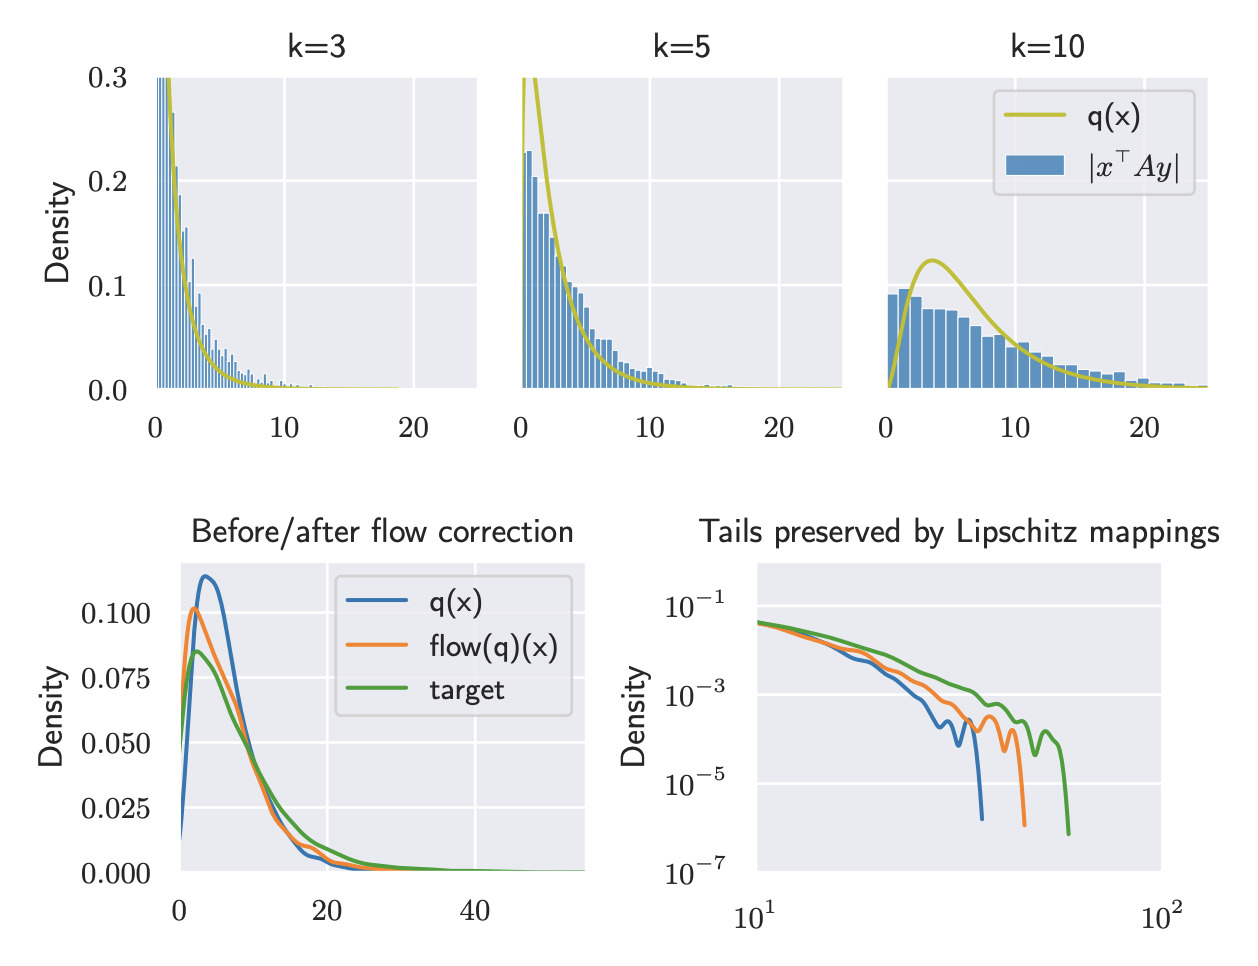
\includegraphics[width=0.7\textwidth]{Figures/gga/flow-correction.png}
		}
	\end{figure}
\end{frame}

\begin{subframe}{Results: variational inference}
    \begin{figure}
        \centering
        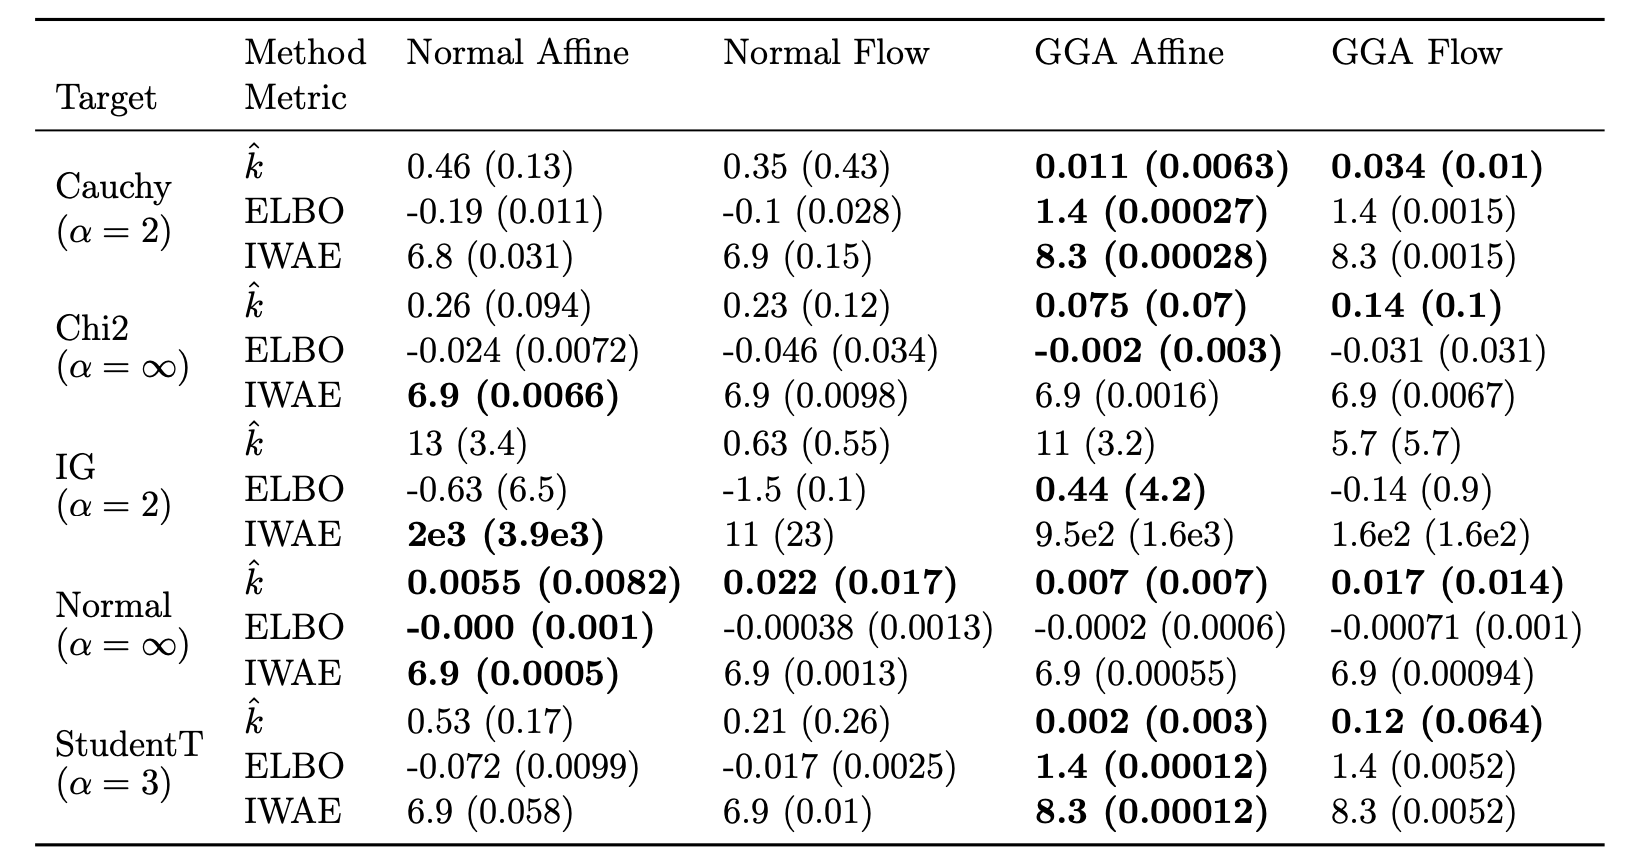
\includegraphics[width=\textwidth]{Figures/gga/vi.png}
    \end{figure}
\end{subframe}

\begin{frame}{Results: density estimation}
    \resizebox{\columnwidth}{!}{%
    \begin{tabular}{llllll}
        \toprule
         & Method & Cauchy ($\alpha=2$) Flow & GGA Affine & GGA Flow & Normal ($\alpha=\infty$) Flow  \\
        Target & Metric &  &  &  &  \\
        \midrule
        \multirow[c]{2}{*}{\shortstack[l]{Cauchy \\($\alpha=2$)}} & $\hat{\alpha}$ & \bfseries 2.1 (0.03) & \bfseries 2.1 (0.04) & \bfseries 2.1 (0.07) & 7.7 (2.5) \\
         & -$H(p,q)$ & \bfseries -2.5e+03 (49) & -3.9e+03 (56) & -3.9e+03 (55) & -1.4e+07 (6.2e+07) \\
         \multirow[c]{2}{*}{\shortstack[l]{IG \\($\alpha=2$)}} & $\hat{\alpha}$ & \bfseries 1.9 (0.03) & \bfseries 1.9 (0.092) & \bfseries 1.9 (0.092) & 7.3 (1.7) \\
         & -$H(p,q)$ & \bfseries -3.5e+03 (83) & -4e+03 (54) & -3.9e+03 (47) & -1.4e+08 (6.2e+08) \\
        \multirow[c]{2}{*}{\shortstack[l]{StudentT \\($\alpha=3$)}} & $\hat{\alpha}$ & 2.0 (0.06) & \bfseries 3.1 (0.16) & \bfseries 3.3 (0.45) & 7.7 (2.3) \\
         & -$H(p,q)$ & \bfseries -2.0e+03 (28) & -3.6e+03 (28) & -3.4e+03 (42) & -3e+03 (4.7e+02) \\
        \multirow[c]{2}{*}{\shortstack[l]{Chi2 \\($\alpha=\infty$)}} & $\hat{\alpha}$ & 2.1 (0.07) & \bfseries 5.5 (1.2) & \bfseries 5.2 (1.6) & \bfseries 6.8 (2.4) \\
         & -$H(p,q)$ & -2.83e+03 (48) &\bfseries -2.76e+03 (26) & -2.80e+03 (44) & -2.85e+03 (38) \\
        \multirow[c]{2}{*}{\shortstack[l]{Normal \\($\alpha=\infty$)}} & $\hat{\alpha}$ & 2.9 (0.6) & \bfseries 8.8 (2.8) & \bfseries 8.2 (4) & \bfseries 8.4 (3.5) \\
         & -$H(p,q)$ &  -1.44e+03 (26) & -1.43e+03 (21) & -1.41e+03 (24) & \bfseries -1.36e+03 (19) \\
        \bottomrule
    \end{tabular}
    }
\end{frame}